\documentclass[12pt,a4paper]{article}
\usepackage[utf8]{vietnam}
\usepackage{amsmath,amssymb}
\usepackage{geometry}
\geometry{top=1.5cm,bottom=1.2cm,left=1.4cm,right=1.4cm,headheight=28pt,headsep=12pt,footskip=18pt}
\usepackage{tikz}
\usepackage{xcolor}
\usepackage{enumerate}
\usepackage{graphicx}
\usepackage[version=4]{mhchem}
\usepackage{fancyhdr}
\usepackage{ex_test}

\renewcommand{\baselinestretch}{0.96}
\setlength{\parskip}{0pt}

\definecolor{hfRed}{RGB}{211,47,47}
\definecolor{hfGreen}{RGB}{139,195,144}

\pagestyle{fancy}
\fancyhf{}
\fancyhead[L]{\small\itshape\color{hfRed} Tài liệu lưu hành nội bộ}
\fancyhead[R]{\small\itshape\color{hfRed} Thầy \textbf{TRẦN VĂN THẠNH} - 0777.470.803}
\renewcommand{\headrulewidth}{0.8pt}
\renewcommand{\headrule}{\hbox to\headwidth{\color{hfGreen}\leaders\hrule height \headrulewidth\hfill}}

\fancyfoot[L]{\small\itshape\color{hfRed} CS1: 6/15 Nguyễn Hoàng, P. Kim Long, TP Huế \quad|\quad CS2: 24 Đặng Thái Thân, TP Huế}
\fancyfoot[R]{\small\bfseries\color{hfRed} Trang \thepage}
\renewcommand{\footrulewidth}{0.8pt}
\renewcommand{\footrule}{\hbox to\headwidth{\color{hfGreen}\leaders\hrule height \footrulewidth\hfill}}

\fancypagestyle{firstpage}{
  \fancyhf{}
  \renewcommand{\headrulewidth}{0pt}
  \fancyfoot[L]{\small\itshape\color{hfRed} CS1: 6/15 Nguyễn Hoàng, P. Kim Long, TP Huế \quad|\quad CS2: 24 Đặng Thái Thân, TP Huế}
  \fancyfoot[R]{\small\bfseries\color{hfRed} Trang \thepage}
  \renewcommand{\footrulewidth}{0.8pt}
  \renewcommand{\footrule}{\hbox to\headwidth{\color{hfGreen}\leaders\hrule height \footrulewidth\hfill}}
}

\begin{document}
\thispagestyle{firstpage}

\noindent
\begin{minipage}[t]{0.44\textwidth}
	\centering\fontsize{10pt}{12pt}\selectfont
	\textbf{SỞ GIÁO DỤC VÀ ĐÀO TẠO THỪA THIÊN HUẾ}\\
	\textbf{ĐỀ CHÍNH THỨC}\\
	\textit{(Đề thi có 04 trang)}
\end{minipage}\hfill
\begin{minipage}[t]{0.54\textwidth}
	\centering\small
	\textbf{ĐỀ KIỂM TRA ĐỊNH KỲ CHƯƠNG 2 (NITROGEN -- SULFUR)}\\
	\textbf{MÔN: HOÁ HỌC -- LỚP 11}\\
	\textit{Thời gian làm bài: 45 phút (không kể thời gian phát đề)}\\
	\fbox{\textbf{MÃ ĐỀ: 104}}
\end{minipage}

\smallskip
\noindent\hrulefill
\smallskip

\noindent\textbf{Họ, tên thí sinh:} \dotfill\ \textbf{Lớp:} \dotfill\ \textbf{Số báo danh:} \dotfill

\smallskip
\noindent\textit{(Cho biết nguyên tử khối: H = 1; C = 12; N = 14; O = 16; Na = 23; Mg = 24; Al = 27; S = 32; Cl = 35,5; Ar = 40; K = 39; Ca = 40; Fe = 56; Cu = 64; Zn = 65; Ba = 137).}
\smallskip

\noindent
\textbf{PHẦN I (4,5 điểm -- 18 câu): Câu trắc nghiệm nhiều phương án lựa chọn.}\\
\textit{Thí sinh trả lời từ câu 1 đến câu 18. Mỗi câu hỏi thí sinh chỉ chọn một phương án.}

\Opensolutionfile{ans}[ans-hoa11-de04hs]

\begin{ex}
Không khí sạch là không khí ít tạp chất chứa các thành phần cơ bản của không khí. Trường hợp nào sau đây được coi là không khí sạch?
\begin{center}
	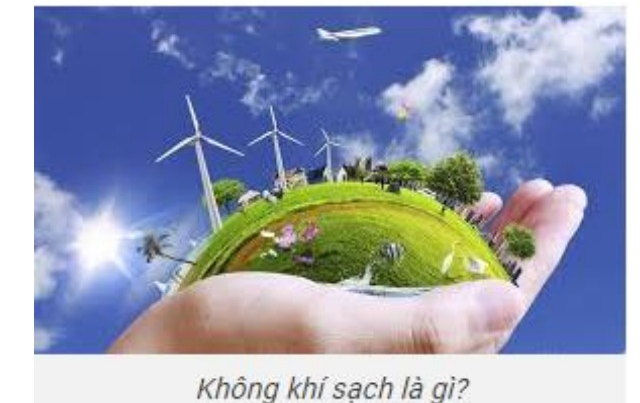
\includegraphics[width=6.5cm]{images_crop_hoa11_de04/cau1_khong_khi_sach.png}
\end{center}
\choice
{Không khí chứa 78\% $\ce{N2}$, 17\% $\ce{O2}$, 3\% $\ce{CO2}$, 1\% $\ce{CO}$, 1\% $\ce{SO2}$.}
{Không khí chứa 78\% $\ce{N2}$, 18\% $\ce{O2}$, 4\% hỗn hợp $\ce{CO2}$, $\ce{SO2}$, $\ce{HCl}$.}
{Không khí chứa 78\% $\ce{N2}$, 20\% $\ce{O2}$, 2\% hỗn hợp $\ce{CO2}$, $\ce{CH4}$ và bụi.}
{Không khí chứa 78\% $\ce{N2}$, 21\% $\ce{O2}$, 1\% hỗn hợp $\ce{CO2}$, $\ce{H2O}$.}
\loigiai{}
\end{ex}

\begin{ex}
\textbf{[CTST - SGK]} Có các loại phân bón như $\ce{NH4Cl}$, $\ce{NH4NO3}$, $\ce{(NH4)2SO4}$, các loại phân bón này không thích hợp bón cho đất nào sau đây?
\choice
{Đất chua}
{Đất phù sa}
{Đất bạc màu}
{Đất nghèo dinh dưỡng.}
\loigiai{}
\end{ex}

\begin{ex}
Biện pháp nào sau đây không hạn chế tình trạng mưa acid?
\choice
{Cho lắp đặt các thiết bị khử sunphua tại những nhà máy nhiệt điện.}
{Loại bỏ nitrogen và sulfur trong dầu mỏ, than.}
{Sử dụng các loại năng lượng có khả năng tái tạo thân thiện với môi trường.}
{Phát tán chất $\ce{NO2}$ và $\ce{SO2}$ vào bầu khí quyển.}
\loigiai{}
\end{ex}

\begin{ex}
\textbf{[KNTT - SBT]} Mưa acid là một thảm họa thiên nhiên toàn cầu, ảnh hưởng đến sự sống của các sinh vật. Mưa acid là hiện tượng mưa có pH
\choice
{$< 5{,}6.$}
{$= 7$}
{$6 - 7.$}
{$> 8.$}
\loigiai{}
\end{ex}

\begin{ex}
\textbf{(SBT - KNTT)} Hiện tượng phú dưỡng là một biểu hiện của môi trường ao, hồ bị ô nhiễm do dư thừa các chất dinh dưỡng. Sự dư thừa dinh dưỡng chủ yếu do hàm lượng các ion nào sau đây vượt quá mức cho phép?
\choice
{Sodium, potassium.}
{Calcium, magnesium.}
{Nitrate, phosphate.}
{Chloride, sulfate.}
\loigiai{}
\end{ex}

\begin{ex}
\textbf{(SBT - KNTT)} Trong số các chất khí: $\ce{SO2}$, $\ce{CO2}$, $\ce{O2}$, $\ce{N2}$, khí tan tốt trong nước ở điều kiện thường là
\choice
{$\ce{O2}$.}
{$\ce{CO2}$.}
{$\ce{SO2}$.}
{$\ce{N2}$.}
\loigiai{}
\end{ex}

\begin{ex}
\textbf{(SBT - CTST)} Dung dịch sulfuric acid đặc khác dung dịch sulfuric acid loãng ở tính chất hoá học nào?
\choice
{Tính base mạnh.}
{Tính oxi hóa mạnh.}
{Tính acid mạnh.}
{Tính khử mạnh.}
\loigiai{}
\end{ex}

\begin{ex}
\textbf{(SBT - KNTT)} Bậc liên kết và năng lượng liên kết trong phân tử nitrogen tương ứng là
\choice
{2 và $418\text{ kJ/mol}$}
{1 và $167\text{ kJ/mol}.$}
{1 và $386\text{ kJ/mol}.$}
{3 và $945\text{ kJ/mol}$}
\loigiai{}
\end{ex}

\begin{ex}
\textbf{(SBT - KNTT)} Xét cân bằng hóa học: $\ce{NH3 + H2O <=> NH4+ + OH-}$. Cân bằng sẽ chuyển dịch theo chiều thuận khi cho thêm vài giọt dung dịch nào sau đây?
\choice
{$\ce{NH4Cl}$.}
{$\ce{NaOH}$.}
{$\ce{HCl}$.}
{$\ce{NaCl}$.}
\loigiai{}
\end{ex}

\begin{ex}
Tính base của $\ce{NH3}$ do nguyên nhân nào sau đây?
\choice
{Trên N còn cặp electron tự do.}
{Phân tử có 3 liên kết cộng hóa trị phân cực.}
{$\ce{NH3}$ tan được nhiều trong nước.}
{$\ce{NH3}$ tác dụng với nước tạo $\ce{NH4OH}$.}
\loigiai{}
\end{ex}

\begin{ex}
$\ce{HNO3}$ đặc thể hiện tính oxi hóa khi tác dụng với chất nào dưới đây?
\choice
{$\ce{Fe2O3}$}
{$\ce{Fe(OH)2}$}
{$\ce{CuCl2}$}
{$\ce{Al2O3}$}
\loigiai{}
\end{ex}

\begin{ex}
Phát biểu nào sau đây sai về $\ce{SO2}$?
\choice
{Chất chống nấm mốc lương thực, thực phẩm.}
{Sản xuất $\ce{H2SO4}$ trong công nghiệp.}
{Không gây ô nhiễm môi trường.}
{Làm chất tẩy trắng giấy và bột giấy.}
\loigiai{}
\end{ex}

\begin{ex}
Nhóm các chất nào sau đây đều tác dụng được với dung dịch $\ce{H2SO4}$ loãng?
\choice
{$\ce{Fe, CuO, Cu(OH)2, BaCl2, NaCl}$.}
{$\ce{FeO, Cu, Cu(OH)2, BaCl2, Na2CO3}$.}
{$\ce{Fe2O3, Cu(OH)2, Zn, Na2SO3, Ba(NO3)2}$.}
{$\ce{Fe(OH)3, Ag, CuO, KHCO3, MgS}$.}
\loigiai{}
\end{ex}

\begin{ex}
Phát biểu nào sau đây sai?
\choice
{$\ce{SO2}$ dùng làm chất tẩy trắng giấy và bột giấy.}
{$\ce{SO2}$ dùng làm chất chống mốc lương thực, thực phẩm.}
{Trong phòng thí nghiệm, $\ce{SO2}$ được điều chế bằng cách đốt quặng pyrit (pyrite).}
{$\ce{SO3}$ là chất trung gian để sản xuất sulfuric acid.}
\loigiai{}
\end{ex}

\begin{ex}
Hiện tượng phú dưỡng là gì?
\choice
{Quá trình tích lũy quá mức các chất dinh dưỡng trong thủy vực, dẫn đến sự phát triển mạnh của thực vật thủy sinh, đặc biệt là tảo.}
{Quá trình thiếu hụt các chất dinh dưỡng trong nước, làm giảm năng suất sinh học của hệ sinh thái.}
{Sự suy giảm chất lượng nước do sự gia tăng vi sinh vật gây bệnh.}
{Hiện tượng mưa acid làm giảm độ pH của nước hồ.}
\loigiai{}
\end{ex}

\begin{ex}
Mưa acid được hình thành khi nào?
\choice
{Khi có sự bốc hơi của nước từ sông hồ.}
{Khi các khí như $\ce{SO2}$ và $\ce{NO_x}$ phản ứng với nước trong khí quyển tạo thành sulfuric acid và nitric acid.}
{Khi các hạt bụi trong không khí kết hợp với nước mưa.}
{Khi carbon dioxide ($\ce{CO2}$) trong không khí phản ứng với nước tạo thành carbonic acid.}
\loigiai{}
\end{ex}

\begin{ex}
Hậu quả chính của mưa acid đối với môi trường là gì?
\choice
{Làm tăng độ pH của nước sông, hồ, gây hại cho hệ sinh thái nước ngọt.}
{Làm tăng lượng chất dinh dưỡng trong đất, giúp cây cối phát triển.}
{Làm giảm độ pH của đất và nước, gây thiệt hại cho cây cối, thủy sinh vật và các tòa nhà.}
{Làm tăng sự phát triển của vi khuẩn trong môi trường đất.}
\loigiai{}
\end{ex}

\begin{ex}
Cho các phát biểu sau:\\
(1) Đối với môi trường, khí sulfur dioxide là nguyên nhân quan trọng gây mưa acid.\\
(2) Chuyển hoá sulfur dioxide thành các chất ít gây ô nhiễm hơn bằng các hóa chất như vôi sống (thành phần chính là $\ce{CaO}$), vôi tôi (thành phần chính là $\ce{Ca(OH)2}$) hoặc đá vôi nghiền (thành phần chính là $\ce{CaCO3}$).\\
(3) Khí sulfur dioxide có màu vàng, ít tan trong nước, thể hiện cả tính oxi hoá và tính khử.\\
(4) Đối với con người, khí sulfur dioxide gây ra cảm giác khó thở, bệnh viêm đường hô hấp, đau mắt.\\
(5) Đơn chất $\ce{N2}$ khó hóa lỏng và tan nhiều trong nước.\\
(6) Tương tác van der Waals giữa các phân tử nitrogen yếu nên khó hóa lỏng.\\
Số phát biểu đúng là
\choice
{3.}
{4.}
{5.}
{6.}
\loigiai{}
\end{ex}

\Closesolutionfile{ans}

\bigskip
\noindent
\textbf{PHẦN II (4,0 điểm -- 4 câu): Câu trắc nghiệm đúng sai.}\\
\textit{Thí sinh trả lời từ câu 1 đến câu 4. Trong mỗi ý a), b), c), d) ở mỗi câu, thí sinh chọn đúng hoặc sai.}

\begin{ex}
Trong phương trình hóa học của phản ứng giữa nitrogen và oxygen:
\choiceTF
{Phương trình hóa học: $\ce{N2 + O2 <=> 2NO}$ (ở $3000^\circ\text{C}$ hoặc tia lửa điện).}
{Oxygen giảm từ 0 xuống -1 $\rightarrow$ oxygen đóng vai trò chất oxi hóa trong phản ứng này.}
{Nitrogen tăng từ 0 lên +4 $\rightarrow$ nitrogen đóng vai trò là chất khử trong phản ứng này.}
{Phản ứng này xảy ra ở nhiệt độ cao trên $3000^\circ\text{C}$ hoặc có tia lửa điện nhưng hiệu suất tạo NO rất thấp nên thực tế không dùng để tạo NO.}
\loigiai{}
\end{ex}

\begin{ex}
Mưa acid gây tác động xấu đến môi trường, con người và sinh vật:
\choiceTF
{Khi nước mưa có pH nhỏ hơn 5,6 thì gọi là hiện tượng mưa acid.}
{Hai tác nhân chính gây mưa acid là $\ce{Cl2}$, $\ce{HCl}$.}
{Mưa acid ăn mòn công trình xây dựng, kiến trúc bằng đá, cẩm thạch và kim loại.}
{Mưa acid làm giảm độ pH của đất và nguồn nước sông hồ, ảnh hưởng nghiêm trọng đến đời sống thủy sinh.}
\loigiai{}
\end{ex}

\begin{ex}
Thành phần chính của khí thiên nhiên là các hydrocarbon như methane (khoảng 80 -- 85\%), ethane, propane, butane cùng lượng nhỏ các khí carbon dioxide, hydrogen sulfide, nitrogen. Thành phần chính của than là carbon, ngoài ra còn có một số hợp chất của các nguyên tố H, S, O, N,...
\choiceTF
{Khi sử dụng khí thiên nhiên hoặc than làm nhiên liệu đều thải vào không khí các chất khí gây ô nhiễm môi trường không khí.}
{Khí thiên nhiên và than khi cháy sẽ toả rất nhiều nhiệt, tạo điều kiện cho các hợp chất như hydrogen sulfide và các hợp chất chứa S, N bị oxi hoá sinh ra các khí độc gây ô nhiễm như $\ce{SO2}$, $\ce{NO}$, $\ce{NO2}$,...}
{Các khí $\ce{SO2}$, $\ce{NO2}$ này là nguyên nhân chính gây ra hiệu ứng nhà kính.}
{Khí thiên nhiên và than đá khi cháy sẽ tạo ra sản phẩm chính là khí $\ce{CO2}$ gây mưa acid.}
\loigiai{}
\end{ex}

\begin{ex}
Khi pha loãng dung dịch $\ce{H2SO4}$ đặc:
\choiceTF
{Sulfuric acid tan tốt trong nước, quá trình hoà tan toả ra một lượng nhiệt lớn.}
{Sulfuric acid tan tốt trong nước, quá trình hoà tan thu một lượng nhiệt lớn.}
{Để đảm bảo an toàn phải cho từ từ nước vào acid và khuấy đều.}
{Để đảm bảo an toàn phải cho từ từ acid vào nước và khuấy đều.}
\loigiai{}
\end{ex}

\bigskip
\noindent
\textbf{PHẦN III (1,5 điểm -- 6 câu): Câu trắc nghiệm yêu cầu trả lời ngắn.}\\
\textit{Thí sinh trả lời từ câu 1 đến câu 6.}

\begin{ex}
Cho sơ đồ chuyển hóa nitrogen trong khí quyển thành phân đạm:
\[\ce{N2 ->[+O2] NO ->[+O2] NO2 ->[+O2 + H2O] HNO3 -> NO3-}\]
Số phản ứng thuộc loại oxi hóa -- khử trong sơ đồ là:

\vspace{1.2cm}

\end{ex}

\begin{ex}
Có bao nhiêu ý kiến sau đây về sulfur dioxide ($\ce{SO2}$) là đúng?\\
(1) Có độc tính đối với con người.\\
(2) Phản ứng được với đá vôi.\\
(3) Khí này được tạo thành từ hoạt động của núi lửa trong tự nhiên, từ quá trình đốt cháy nhiên liệu hóa thạch của con người,...\\
(4) Là oxide lưỡng tính.

\vspace{1.2cm}

\end{ex}

\begin{ex}
Tính thể tích ($\text{mL}$) dung dịch $\ce{H2SO4}\ 98\%$ (khối lượng riêng $D = 1{,}84\text{ g/mL}$) cần dùng để pha chế thành $500\text{ mL}$ dung dịch $\ce{H2SO4}\ 0{,}05\text{ M}$ (làm tròn đến hai chữ số phần thập phân).

\vspace{1.2cm}

\end{ex}

\begin{ex}
\textbf{(SBT - KNTT)} Tính phân tử khối trung bình của không khí, giả thiết thành phần không khí gồm: $78\%$ nitrogen, $21\%$ oxygen và $1\%$ argon (làm tròn kết quả đến phần nguyên).

\vspace{1.2cm}

\end{ex}

\begin{ex}
Hỗn hợp X gồm $\ce{N2}$ và $\ce{H2}$ có khối lượng mol trung bình $\overline{M}_X = 12{,}4\text{ g/mol}$. Dẫn X đi qua bình đựng bột Fe rồi nung nóng (hiệu suất tổng hợp $\ce{NH3}$ đạt $40\%$), thu được hỗn hợp Y. Giá trị khối lượng mol trung bình $\overline{M}_Y$ là bao nhiêu $\text{g/mol}$? (làm tròn kết quả đến hàng phần mười).

\vspace{1.2cm}

\end{ex}

\begin{ex}
Một khu vực nông nghiệp gần hồ có diện tích $10\text{ km}^2$, hằng năm lượng nước chảy tràn từ mưa cuốn theo phân bón vào hồ chứa khoảng $5\text{ mg/L}$ nitrate ($\ce{NO3-}$). Nếu lượng nước chảy tràn chiếm $2\%$ lượng mưa, và lượng mưa trung bình hàng năm là $800\text{ mm}$, tính khối lượng nitrate (theo đơn vị $\text{kg}$) bị thải vào hồ mỗi năm.

\vspace{1.2cm}

\end{ex}

\bigskip
\noindent
\textbf{PHẦN IV: Tự luận}\\
\textit{Học sinh giải chi tiết các câu hỏi sau vào giấy làm bài.}

\begin{ex}
\textbf{(SBT - CD)} Trong quy trình sản xuất tơ, mỗi năm có hàng triệu tấn cyclohexanone ($\ce{C6H10O}$) được cho phản ứng với $\ce{HNO3}$ để tạo adipic acid ($\ce{C6H10O4}$) theo phản ứng:
\[\ce{C6H10O + HNO3 -> C6H10O4 + N2O + H2O}\]
a) Cân bằng phương trình hoá học của phản ứng trên theo phương pháp thăng bằng electron.\\
b) Cho biết vai trò của $\ce{HNO3}$ trong phản ứng trên. Giải thích.

\vspace{2.5cm}

\end{ex}

\begin{ex}
\textbf{(SBT - CTST)} Muối $\ce{NH4NO3}$ sẽ nhiệt phân theo phản ứng nào trong 2 phản ứng sau? Giải thích.
\begin{align*}
	\ce{NH4NO3(s) &->[t^\circ] NH3(g) + HNO3(g)} \tag{1} \\
	\ce{NH4NO3(s) &->[t^\circ] N2O(g) + 2H2O(g)} \tag{2}
\end{align*}
Biết enthalpy tạo thành chuẩn $\Delta_f H^\circ_{298}\ (\text{kJ/mol})$ của các chất như sau:
$\ce{NH4NO3(s)}: -365{,}61$; $\ce{NH3(g)}: -45{,}90$; $\ce{N2O(g)}: 82{,}05$; $\ce{HNO3(g)}: -134{,}31$; $\ce{H2O(g)}: -241{,}82$.

\vspace{3.5cm}

\end{ex}

\begin{center}
\textbf{--------- HẾT ---------}
\end{center}

\end{document}
